
\chapter{System Architecture}

\section{Drone}
Drones (quadcopters) are the most extensively used versions of Unmanned Aerial Vehicles (UAVs) in various fields due to their high maneuverability and stability in almost every condition. This results in their widespread use in field of applications entailing high flight times, high altitudes, stable operation and communication. We explored 3 different flight controllers for drone maneuvering, explained in the coming sections. We also developed a code to maneuver drones in a constrained environment from scratch through python based communication over WiFi for the PID controls, processing on base station (Laptop) and waypoint navigation with obstacles through Lua Scripting on Open Licensed version of Virtual Robotic Simulator V-REP simulator and emulator. This used an overhead camera to understand the dynamics of drones in aerodynamic range as well as exploited the RF communications. We further used CC3D mini flight controller to fly the drone using in built codes, calibrating the ESCs and the flight controller with the motors on the custom chassis drone we developed the architecture of. We then moved to the APM 2.8 flight controller to incorporate the GPS control and telemetry extensions. We used Mission Planner to plan the path using a polygon method where the planner automatically divides the whole region in smaller paths at given altitude and covers the entire polygon. The Open Drone Map Plugin in Mission planner triggers the data acquisition circuitry to click images and later stitch the orthomosaic. 

\subsection{Waypoint Navigation in constrained environment}
We experimented on the Pluto X drone developed by Dronaviation to understand the dynamics of drone by coding it from scratch to implement the PID algorithm (Propotional-Integral-Derivative Controller algorithm). 
\begin{figure}[H]
    \centering
    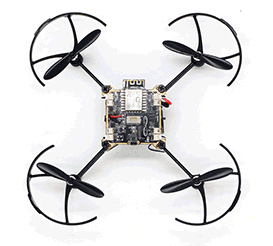
\includegraphics[]{SummerInterReport/project/Images-Major/plutox.png}
    \caption{PlutoX drone from dronaaviation}
    \label{fig:plutox}
\end{figure}
The plutoX drone has the Primus V3R flight controller. It has 16 GPIOs, 2 DAC (Digital to Analog Converter) Channels, 10 DOF (Degrees Of Freedom) Sensor Suite, 4 Mosfet Drivers, 2 UARTs, 20 Pin Header, 4 H Bridge Drivers to connect the Brushless DC motors and 11 Timer Channels. The drone practically presents a 10 minutes flight time with an 800 mAh Lithium Polymer 27C (Lipo battery) with a charge time of 45 minutes. The board has an on-board WiFi module which allows it to communicate over a distance of 60m with any WiFi module operating on 802.11ac protocols. 
\\
\\
We use the whole setup in a constrained environment where we are limited by the vision of an overhead camera. For the task of simple waypoint navigation, we present a WhyCon coordinate. The WhyCon is a vision-based localization system that can be used with low cost web cameras. It achieves millimeter precision with very high performance. These markers consist of a dark outer ring and a concentric white circle. The WhyCon coordinate is basically the position of presence of the marker in the camera, in its own frame of reference. They are detected through the overhead camera using the open source WhyCon Robotics Operating System package over the ROS environment. In addition to the final waypoint destination being marked using a Whycon, the drone is also detected in the scene using WhyCon detection. It is affixed with a WhyCon marker on its top which helps in identifying its position and thus localize it in the frame. The overhead camera is connected to the central processor, Laptop, using wired USB connection and the drone is connected through WiFi.
\begin{figure}[H]
    \centering
    \includegraphics[scale=0.6]{SummerInterReport/project/Images-Major/WhyCon_plutox.png}
    \caption{PlutoX drone with WhyCon Marker schematic}
    \label{fig:plutox_WhyCon}
\end{figure}
We calculate the error of the drone's current position, as given by the currently detected WhyCon coordinates of drone from the overhead camera, compared to the final waypoint's position. This error is fed to the PID controller in derivative, current and iterative sum form. The PID controller algorithm we developed finds the throttle, pitch and yaw values to be given to the drone to make it traverse to the given waypoint. The given four channel values are relayed to the drone by the laptop as RC commands from the RC WiFi communication built by the drone.
\\
\begin{figure}[H]
    \centering
    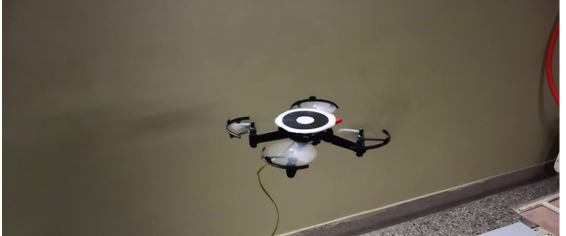
\includegraphics[]{SummerInterReport/project/Images-Major/Flying_pluto.png}
    \caption{PlutoX drone mid-flight}
    \label{fig:plutox_flying}
\end{figure}


The complete experimental setup is made such that the drone employs a WhyCon marker over it for the camera to identify. The environment is populated with Hula hoops through which the drone has to pass with given positions and orientations. The positions of the hoops are set-up initially via the WhyCon markers affixed on the hoops and the orientations are setup via the Aruco markers. ArUco marker is a 5x5 grid that is black and white in color and are based on Hamming code. They can have the position as well an orientation attribute computed with respect to the overhead camera.
\\
The Overhead camera has a fish-eye effect which is corrected using chess-board camera calibration method. The corrected coordinates present are in the following form:
\begin{figure}[H]
    \centering
    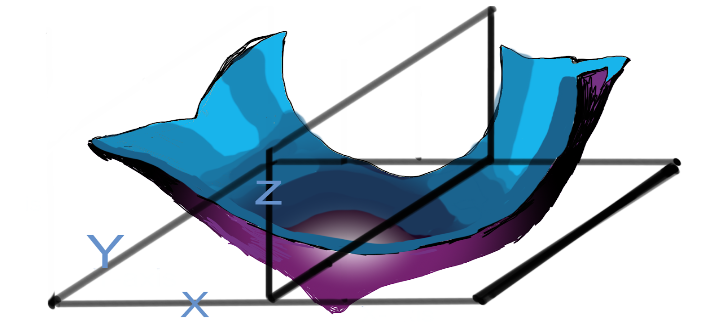
\includegraphics[scale=0.6]{SummerInterReport/project/Images-Major/varz.png}
    \caption{Variation in Z-axis with respect to x-y plane}
    \label{fig:varz}
\end{figure}
\begin{table}[H]
    \centering
    \begin{tabular}{|c|c|}
     \hline
     \textbf{Position} & \textbf{WhyCon Z Coordinate}  \\
     \hline
     Centre & 33.47\\
     Top-left & 29.80\\
     Top-right & 30.82\\
     Bottom-left & 29.42\\
     Bottom-right & 29.58\\
     \hline
    \end{tabular}
    \caption{Variation of Z axis with x-y plane}
    \label{tab:varz}
\end{table}

The python code identifies the positions and orientations of the hoops using WhyCon markers and ArUco markers respectively and sends the same over ROS to the Coppepelia Robotics' Virtual Robotics simulator, V-REP (Virtual Robotics Emulation Platform). The Lua Script developed in the V-REP environment uses these positions and orientations and convert them to V-REP's global frame of reference using mathematical models.\\

The lua script then places the hoops and the obstacles (in similar way) in the virtual scenario, thereby emulating the real world scenario. It then devises the path to the hoops sequentially. Each hoop is taken as a final waypoint by the drone. The Lua code uses RRTConnect polygon based algorithm to find the path from the initial waypoint to the final waypoint. THe path is computed so that there must be no collision with the obstacles. This is achieved by making collision pairs between the drone, the obstacles and the hoop bodies in the 6D state space defined in the Virtual scene itself. The computed random optimum path between the initial waypoint and the final waypoint results in several intermediate waypoints. This reduces the task to the basic waypoint navigation problem, where the drone computes error vectors and stabilize at a given waypoint. After a threshold of stability and proximity to the designated intermediate waypoint, we supply the next waypoint to be followed, thereby, completing the whole path. Similarly, once a path is completed, the past final waypoint now becomes its current initial point and the next hoop's position becomes the final waypoint. 
\\

The setting up of each stage is explained through flowcharts in the following. Hoops are called trees here.
\begin{figure}[H]
    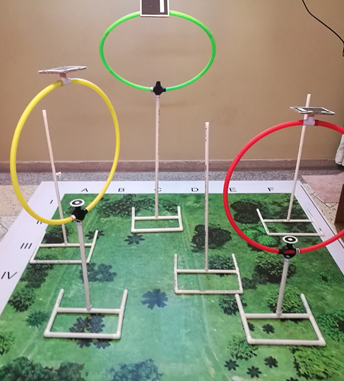
\includegraphics[scale=0.9]{SummerInterReport/project/Images-Major/arena.png}
    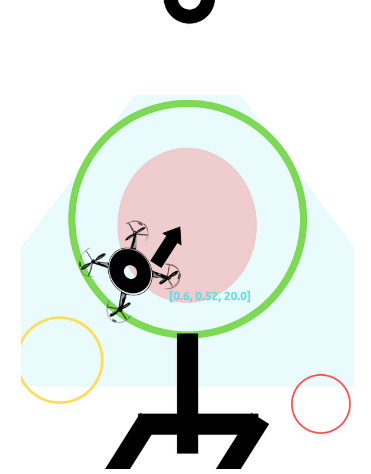
\includegraphics[scale=0.9]{SummerInterReport/project/Images-Major/eyflow.png}
    
    \caption{L: Arena Image with hoops and obstacles; R: Overhead camera and hoop navigation}
    \label{fig:arena}
\end{figure}
\large{\textbf{PID Code Snippet (Python)}}
\begin{lstlisting}[language=Python]
def pid(self):
		self.currenttime=time.time()#Takes the current time stamp
		self.error=[a1-b1 for a1,b1 in zip(self.drone_position,self.setpoint)]#Calculates the error by subtracting drone position and set waypoint positions
		self.sum_values=[a1+b1 for a1,b1 in zip(self.sum_values,self.error)]#sum of previous error values are added together for the given sample time
		if(self.currenttime-self.lasttime>=self.sample_time):
			# If the sample time has elapsed, tune PID
			self.dif_error= [a1-b1 for a1,b1 in zip(self.error,self.prev_error)]#derivative term- difference between current and previous error
			#Pitch, Roll, Throttle and Yaw are calculated with PID formulas
			self.cmd.rcPitch=int(1500 + (self.error[1]*self.Kp[0]+self.dif_error[1]*self.Kd[0]/(self.sample_time)+self.sum_values[1]*self.Ki[0]*self.sample_time/self.iterations))
			self.cmd.rcRoll=int(1500 - (self.error[0]*self.Kp[1]+self.dif_error[0]*self.Kd[1]/(self.sample_time)+self.sum_values[0]*self.Ki[1]*self.sample_time/self.iterations))
			self.cmd.rcThrottle=int(1500 + self.error[2]*self.Kp[2]+self.dif_error[2]*self.Kd[2]/(self.sample_time)+self.sum_values[2]*self.Ki[2]*self.sample_time/self.iterations)
			self.cmd.rcYaw=int(1500-(self.error[3]*self.Kp[3]+self.dif_error[3]*self.Kd[3]/(self.sample_time)+self.sum_values[3]*self.Ki[3]*self.sample_time/self.iterations))
			self.lasttime=self.currenttime#The last time stamp is updated
self.prev_error=self.error#Previous error term is updated
\end{lstlisting}


\begin{figure}[H]
    \centering
    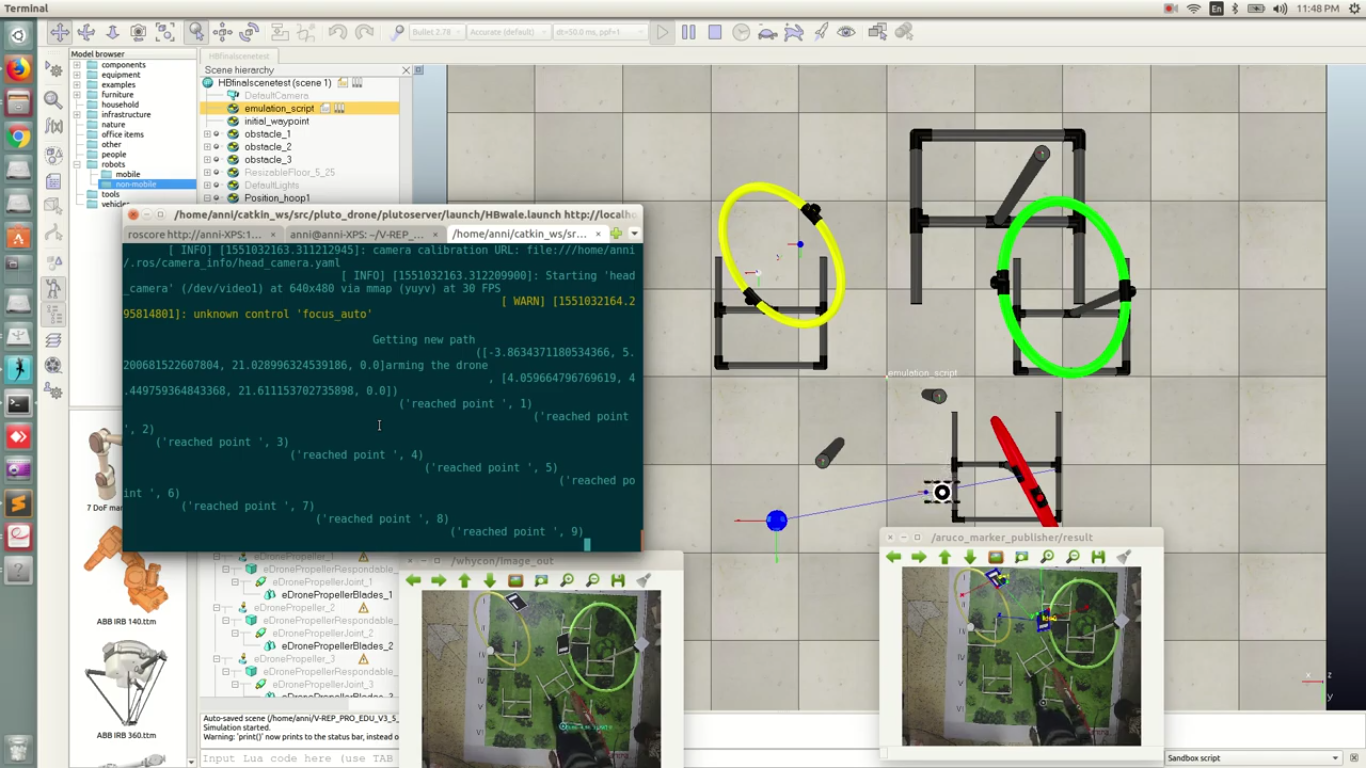
\includegraphics[width=\linewidth]{SummerInterReport/project/Images-Major/simul.png}
    \caption{Simulation and Emulation in V-REP}
    \label{fig:simul}
\end{figure}
\begin{figure}[H]
    \centering
    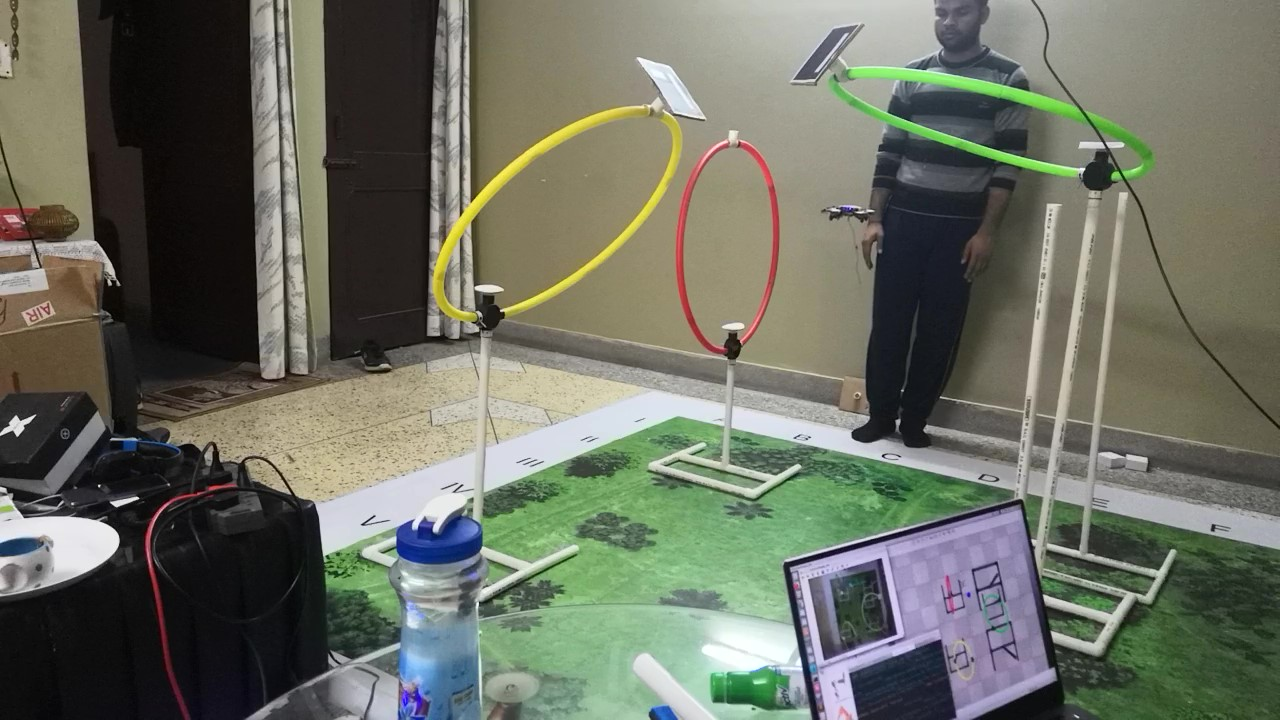
\includegraphics[width=\linewidth]{SummerInterReport/project/Images-Major/finalarena.jpeg}
    \caption{Traversal of PlutoX through designed arena}
    \label{fig:simul}
\end{figure}
\begin{figure}[H]
    \centering
    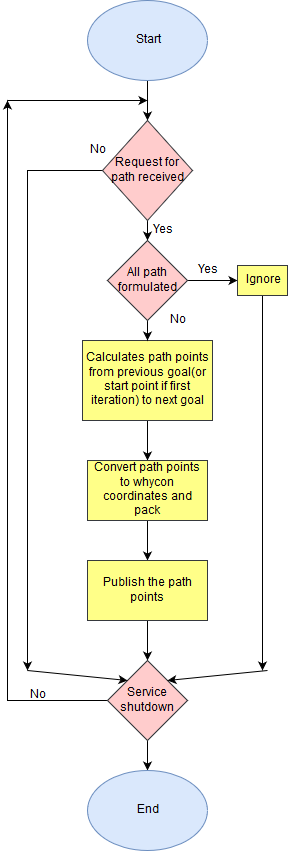
\includegraphics[]{SummerInterReport/project/Images-Major/pathplan.png}
    \caption{Path planning in Lua Script}
    \label{fig:pathPlan}
\end{figure}

\begin{figure}[H]
    \centering
    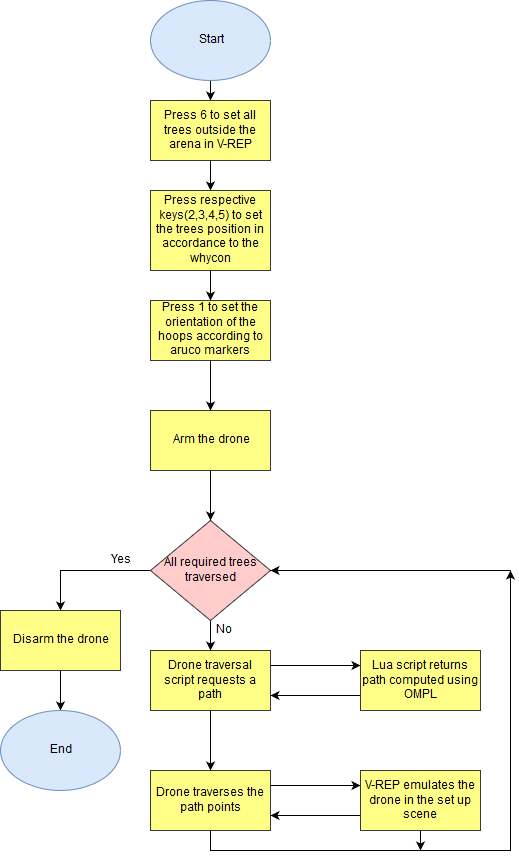
\includegraphics[]{SummerInterReport/project/Images-Major/completeEy.png}
    \caption{Complete experimental flow of constrained waypoint navigation}
    \label{fig:compEy}
\end{figure}

\subsection{PID Tuning - Mathematics}
Systems can broadly be divided into two types; \textbf{open loop systems} and \textbf{closed loop systems}. An open loop system, also called an uncontrolled system, is one in which there is no feedback from the output of the system to the input. A closed loop system on the other hand is a controlled system which has receives a feedback of its operation at every point of time. PID (Proportional-integral-derivative) Controllers are a type of close loop systems. They are used widely in automation industries, aviation industries and other technologies where a feedback is required due to their robust nature covering a diverse range of operations and the ease with which they are implemented. They can be used in any application which requires a feedback mechanism to take control of the rise times, over-shootings, steady-state errors and oscillations damping.
\\
\textbf{Types of Controllers}
\begin{itemize}
    \item \textbf{Proportional Controller (P Controller)} \\
    P controller is mostly used in first order processes with single energy storage to stabilize the unstable process. The main usage of the P controller is to decrease the steady state error of the system. As the proportional gain factor K increases, the steady state error of the system decreases. However, despite the reduction, P control can never manage to eliminate the steady state error of the system. As we increase the proportional gain, it provides smaller amplitude and phase margin, faster dynamics satisfying wider frequency band and larger sensitivity to the noise. We can use this controller only when our system is tolerable to a constant steady state error. In addition, it can be easily concluded that applying P controller decreases the rise time and after a certain value of reduction on the steady state error, increasing K only leads to overshoot of the system response. P control also causes oscillation if sufficiently aggressive in the presence of lags and/or dead time. The more it lags (higher order), the more problem it leads. Plus, it directly amplifies process noise. 
    \item \textbf{Proportional Derivative Controller (PD Controller)} \\
    The aim of using P-D controller is to increase the stability of the system by improving control since it has an ability to predict the future error of the system response. In order to avoid effects of the sudden change in the value of the error signal, the derivative is taken from the output response of the system variable instead of the error signal. Therefore, D mode is designed to be proportional to the change of the output variable to prevent the sudden changes occurring in the control output resulting from sudden changes in the error signal. In addition D directly amplifies process noise therefore D-only control is not used.
    \item \textbf{Proportional Integral Derivative (PID Controller)}\\ P-I-D controller has the optimum control dynamics including zero steady state error, fast response (short rise time), no oscillations and higher stability. The necessity of using a derivative gain component in addition to the PI controller is to eliminate the overshoot and the oscillations occurring in the output response of the system.
\end{itemize} 
\\
\textbf{Equations and Diagrams}
\begin{enumerate}
    \item \textbf{P controller}\\
    A P controller consists of only a linear gain Kp. The output of such controller can be simply given as\\
    \begin{equation}
        output = Kp * error
    \end{equation}
    \begin{figure}[H]
        \centering
        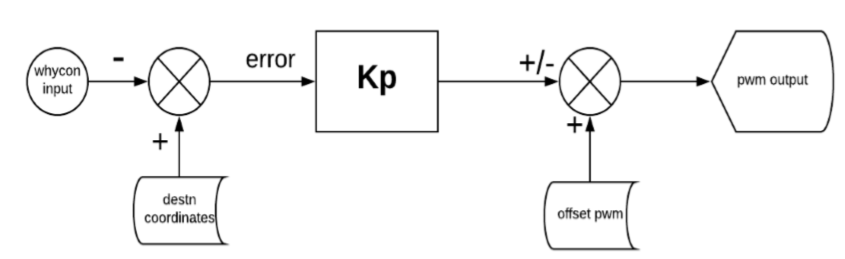
\includegraphics[width=0.8\linewidth]{SummerInterReport/project/Images-Major/pblock.png}
        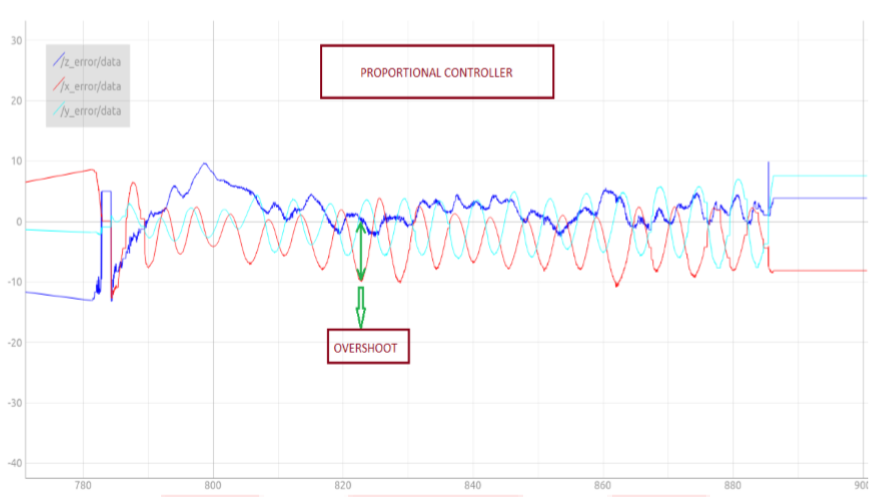
\includegraphics[width=0.8\linewidth]{SummerInterReport/project/Images-Major/pgraph.png}
        \caption{P controller Block Diagram and Graph}
        \label{fig:Pcontroller}
    \end{figure}
    The WhyCon input consists of x, y and z coordinates which gives the current location of the drone. Suppose the destination is say, (x1, y1, z1), then the difference of coordinates i.e (x1-x) ,(y1-y), (z1-z) will be fed as an input to the P-controller. The resultant product i.e Kp * error will be added or subtracted to the offset pwm as the need be to give the final output.
    
    \item \textbf{PD Controller}\\
    Oscillations can be damped by using a differential gain along with the P-Controller. The system as a whole is said to be a PD Controller.
    \begin{figure}[H]
        \centering
        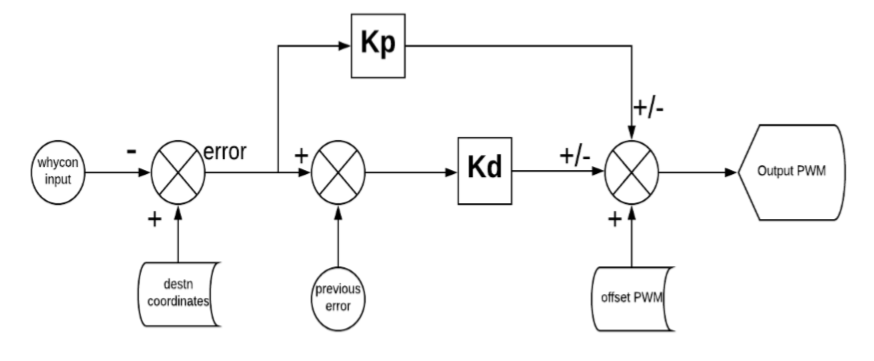
\includegraphics[width=0.8\linewidth]{SummerInterReport/project/Images-Major/dblock.png}
        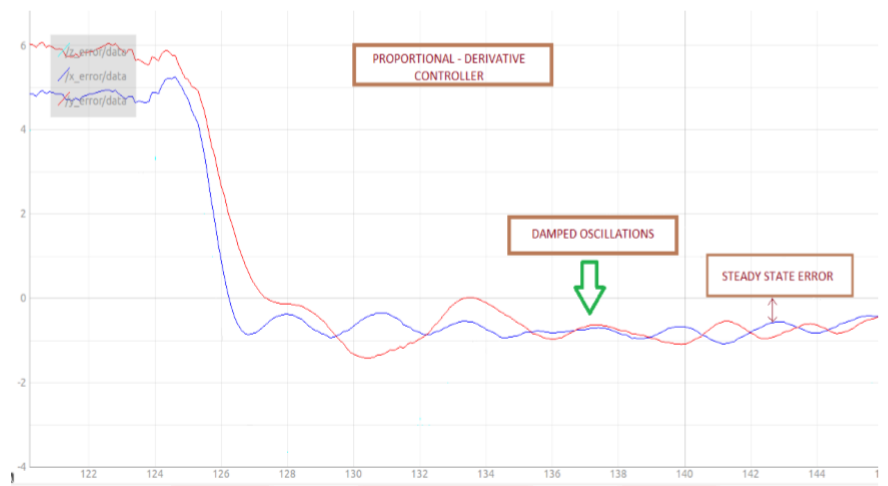
\includegraphics[width=0.8\linewidth]{SummerInterReport/project/Images-Major/dgraph.png}
        \caption{PD controller Block Diagram and Graph}
        \label{fig:PDcontroller}
    \end{figure}
    The differential gain Kd is multiplied with the difference of error and previous error. Previous error is a variable that holds the last error generated by the controller output.\\
    The controller output in this case is given as
    \begin{equation}
        output = Kp * error + Kd * (error - previous error)
    \end{equation}
    Note that Kd is calculated keeping the sampling time in consideration. This output will be further added or subtracted to the offset pwm as the need be to give the final output.
    
    \item \textbf{PID Controller}\\
        In order to minimise the steady state error we introduce another gain called Ki ,the integral gain. Such a system is said to be a PID Controller
        \begin{figure}[H]
        \centering
        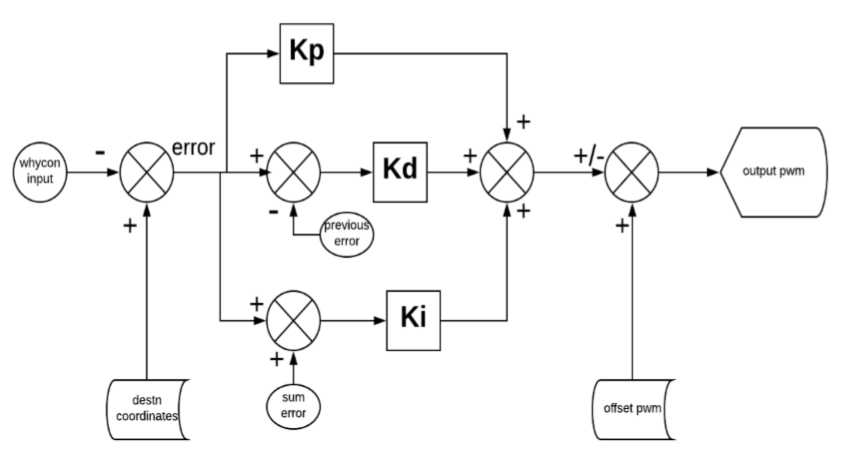
\includegraphics[width=0.8\linewidth]{SummerInterReport/project/Images-Major/pidblock.png}
        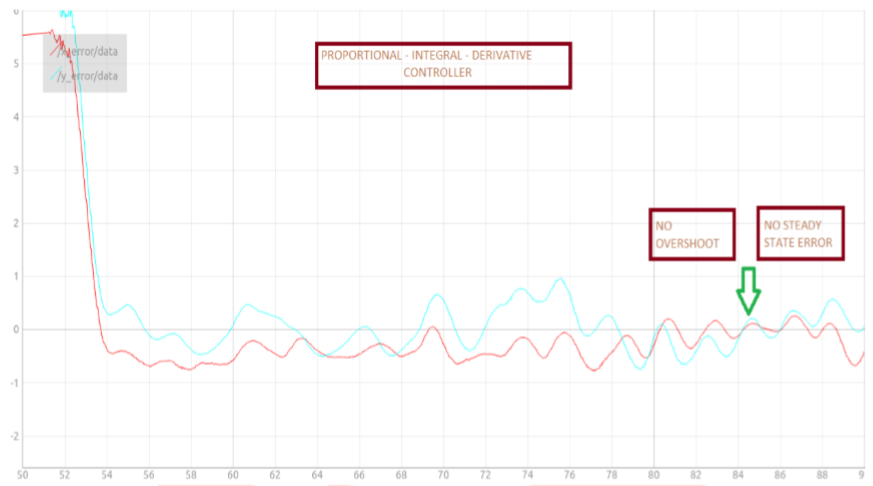
\includegraphics[width=0.8\linewidth]{SummerInterReport/project/Images-Major/pidgraph.png}
        \caption{PID controller Block Diagram and Graph}
        \label{fig:PIDcontroller}
    \end{figure}
    Here in we keep track of the error over time i.e. sum up the errors over a specified sampling time.
    \begin{equation}
        Iterm = (Iterm + error) * Ki
    \end{equation}
    Note that Ki is calculated keeping the sampling time in consideration. This output will be further added or subtracted to the offset pwm as the need be to give the final output.
    \begin{equation}
        output = Kp*error + Iterm + Kd*(error - previous error)        
    \end{equation}


\end{enumerate}


















\subsection{Drone architecture and components}
In order to successfully navigate through the field, we need to ensure a drone with all the parts intact which are distinctive for each size of the drone. We have used the 250mm or the 25cm Carbon Fiber Chassis of the drone to build a sturdy, powerful and small drone, capable of doing everything with lesser power utilization, greater flight times and better handling at constrained areas. We use the quad-copter in X-copter fashion, meaning that two peds of the quad-copter would face the front hen we give it a pitch and a X orientation is followed at all times, no individual leg leans on giving it pitch, roll or yaw. 
\begin{figure}[H]
    \centering
    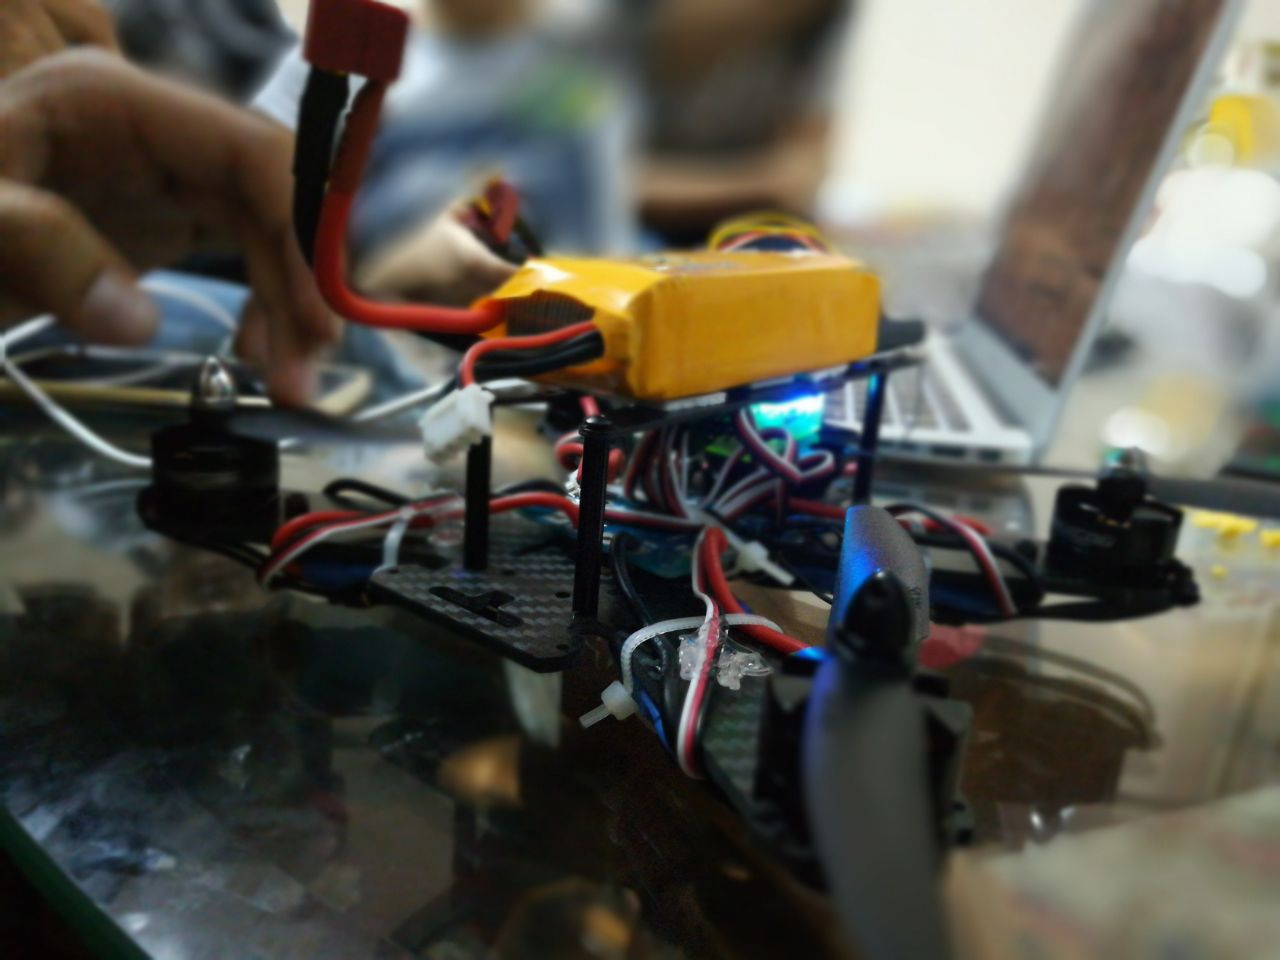
\includegraphics[width=0.8\linewidth]{SummerInterReport/project/Images-Major/drone.jpeg}
    \caption{Custom 250mm drone}
    \label{fig:drone}
\end{figure}
The components used are-
\\
\begin{enumerate}
    \item \textbf{Standard Prop}\\
    The propellers are specifically designed wings of the drone. The propeller design is based on the direction of the circular motion, either it is clockwise or anti-clockwise. The propellers are made from high grade plastics to avoid breaking on crashes. They have an aerodynamic body due to a lean in their horizontal axis to either inwards or outwards based on which, they are fixed on Clockwise or Counter Clockwise motors. The lean is such that the propellers always push air in a downward direction when fixated on the designated clockwise or the anticlockwise motor. This provides necessary thrust for the drone to take off, increase altitude or change its direction. We have used both Two Blade and Three-bladed propellers of 2.2cm single wing span.
    \item \textbf{Brushless DC Motors (BLDC Motors)}\\
    We used high power (2200 kV) brush less DC motors in order to levitate the drone along with the body and attachment payload. To make a drone fly, the rotation of all the motors should oppose the rotation to the adjacent motors. The given motors were connected specifically to the clockwise and counter-clockwise directions.
    \begin{figure}[H]
    \centering
    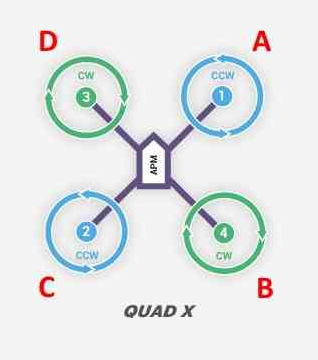
\includegraphics[]{SummerInterReport/project/Images-Major/motors.png}
    \caption{Drone BLDC motor connections}
    \label{fig:motors}
\end{figure}
    \item \textbf{Electronics Speed Controllers(ESC)}\\
    An electronic speed controller or ESC is an electronic circuit with the purpose to vary an electric motor's speed, its direction and possibly also to act as a dynamic brake. It converts DC battery power into 3-phase AC for driving brushless motors. It offers high power, high frequency, high resolution 3-phase AC power to the motors in an extremely compact miniature package. We used Rapid ESCs with high current ratings (3A) to drive the motors. They basically act as the motor driver circuits in drone with PWM signalling in rapid fashion. The ESC gets power from the LiPo battery and have a signalling wire as well.
    \item \textbf{Battery}\\ 
    We used Lithium polymer (LiPo) batteries, It offers the best combination of energy density and power density. It also gives the optimal flight time to cover the planned area. The LiPo battery we used had a 2200 mAh capacity with a 20C rating.
    \item \textbf{Power Distribution Board}\\
    It acts as the intermediary between the LiPo battery, the ESCs and the other electronic circuitry like GPS, receivers and the flight controller on board the drone.
    \item \textbf{Transmitter-Receiver or GPS}\\
    These are used to give direction to the drone. We initially used a FlySky transmitter-Receiver at 2.4 GHz for manually giving the 6 channel input (including throttle, pitch, roll and yaw) commands to the drone. For automated controls, a GPS was used along with Mission Planner software to plan the path and burn this updated firmware into the flight controller for it to follow the path. 
    \item \textbf{Flight Controller} \\
    We tried using CC3D Mini as well as APM2.8, both of which are discussed below
\end{enumerate}

\begin{figure}[H]
    \centering
    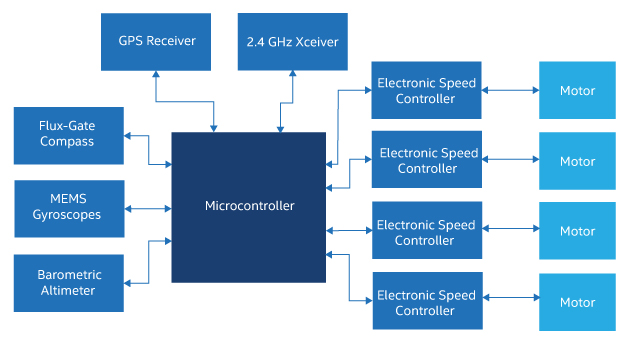
\includegraphics[]{SummerInterReport/project/Images-Major/block.png}
    \caption{Architecture Overview from System Design Journal - Intel us-system design-journal-drones-f1}
    \label{fig:compEy}
\end{figure}


\subsection{CC3D mini Flight Controller}
The CopterControl, CC3D and mini CC3D flight controllers are all types of stabilisation hardware which run the OpenPilot firmware. They can be configured to fly any air-frame from fixed wing to an octocopter using the OpenPilot Ground Control Station (GCS) software. The CopterControl was the first generation board, which ceased manufacture in 2012 due to lack of availability of the gyro sensors used for stabilisation. The board design was then revised and released with an improved gyro sensor which is less affected by temperature changes. This revision is called the CC3D, and apart from the gyro sensor change is identical to the original CopterControl.
\\
We used the CC3D Mini board which is as cheap as Rs 700 or 10\$ and contains the firmware to fly the drone manually using a transmitter-receiver. GPS cannot be integrated with this flight controller, hence we depreciated it of its use in our work. 

\begin{figure}[H]
    \centering
    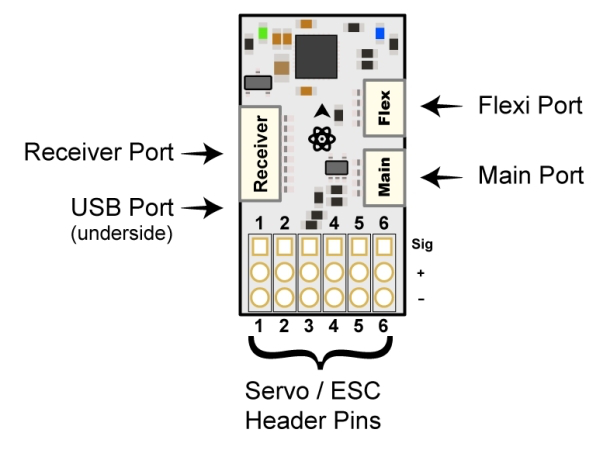
\includegraphics[scale=0.35]{SummerInterReport/project/Images-Major/cc3d.png}
    \caption{Schematic of mini cc3d (Source: DroneTrest)}
    \label{fig:compEy}
\end{figure}
\subsection{APM 2.8 Flight Controller}
Ardupilot Mega (APM) is a professional quality IMU autopilot that is based on the Arduino Mega platform.  This autopilot can control fixed-wing aircraft like drones, multi-rotor helicopters, as well as traditional helicopters.  It is a full autopilot capable for autonomous stabilisation, way-point based navigation and two way telemetry with Xbee wireless modules. It supports 8 RC channels with 4 serial ports. It is our main choice of Flight controller due to it's \textbf{advancements over the CC3D mini.}
\\
It is an open source autopilot firmware that supports planes, multicopters with full mission scripting over point-and-click. It Can support hundreds of 3D waypoints and also Autonomous takeoff, landing and special action commands such as video and camera controls. There is presence of automatic modes like loitering, stabilization, altitude-hold, Return-To-Launch over manual control and accurate GPS waypoint mapping in autonomous conditions.
\\
Ardupilot works on the ArduCopter 5.3.3 firmware which is installed with the help of mission planner. The firmware is the code that runs on the board as a permanent embedded software. Depending on what code we load, we can use the APM to control fixed wing aircraft, multi rotors, helicopters and also ground rovers. We use ArduPilot Mission Planner to update the firmware on the board. The APM board is based on Atmega2560 chip with a small on-board flash memory of 128kB and 16kBs of RAM.
\\ 
The APM 2.8 Board has extension ports for Telemetry, External I2C port, Old and New GPS port, a USB port for uploading the firmware and mission, and other GPIO pins as well to support expandability.

\begin{figure}[H]
    \centering
    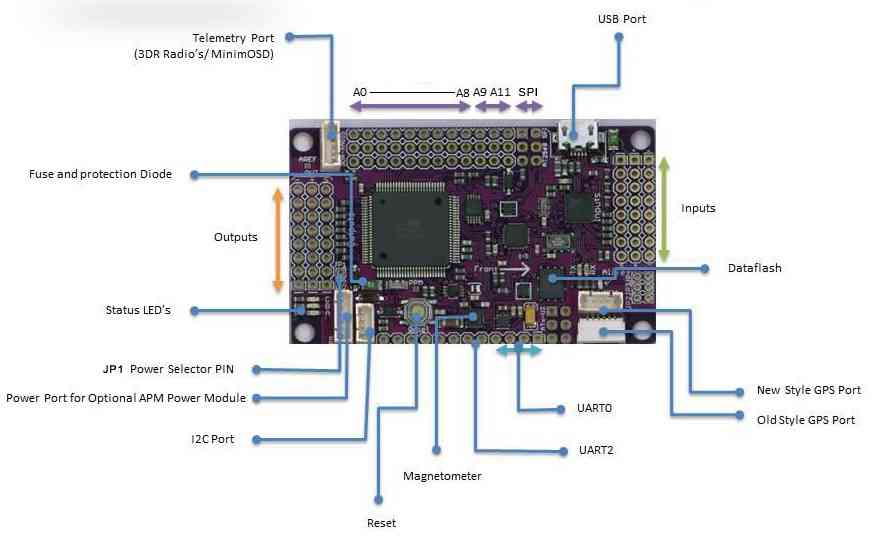
\includegraphics[scale=0.7]{SummerInterReport/project/Images-Major/apm.jpg}
    \caption{Schematic of APM2.8 (Source: ArduPilot)}
    \label{fig:apm}
\end{figure}
\subsection{GPS and Mission Planner}
For navigation of drone and monitoring the field, we use Ublox M8N GPS module. which is highly sensitive and its gives highly accurate position of the navigating drone. The GPS module is high precision and gives low errors to ensure safe flight. It is used for reaching the given point as well as mapping the whole area and covering it.
\\
Mission Planner is a ground control station for Plane, Copter and Rover. It is compatible with Windows only. Mission Planner can be used as a configuration utility or as a dynamic control supplement of the autonomous vehicle. For initial setup-
\begin{enumerate}
    \item Load the firmware (the software) into the APM2.8
    \item Setup, configure, and tune the motors and ESCs of the Drone and the transmitter controls.
    \item Plan, save and load autonomous missions into autopilot with simple point-and-click way-point entry on Google or other maps.
    \item Download and analyze mission logs created by autopilot.
    \item Interface with a PC flight simulator to create a full hardware-in-the-loop UAV simulator.
\end{enumerate}

With appropriate telemetry hardware, we can also Monitor drone status while in operation and record telemetry logs which contain much more information of the on-board autopilot logs. 
\begin{figure}[H]
    \centering
    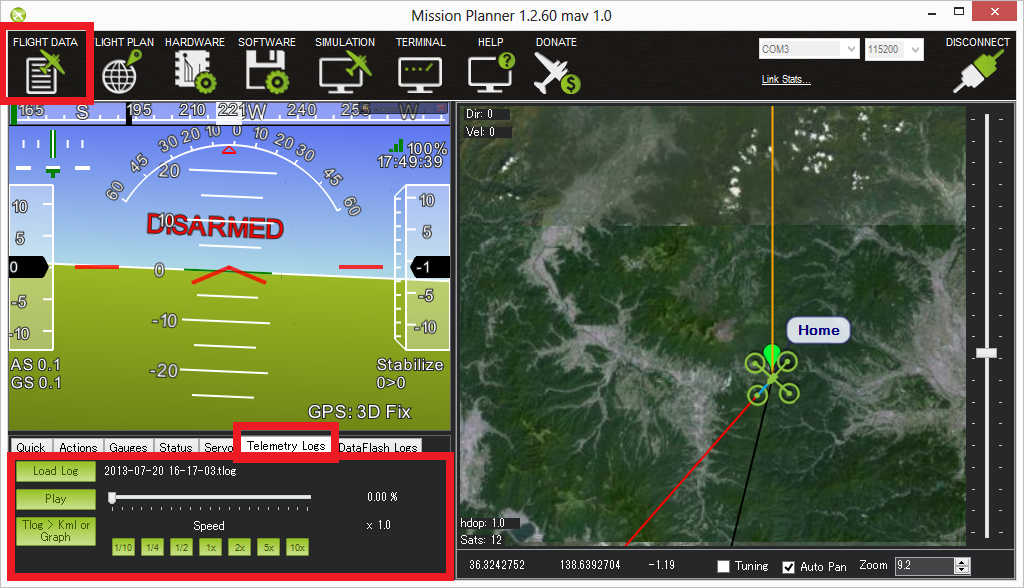
\includegraphics[width=\linewidth]{SummerInterReport/project/Images-Major/mp1.png}
    \caption{Mission Planner GUI(Source: ardupilot.org)}
    \label{fig:compEy}
\end{figure}

\begin{figure}[H]
    \centering
    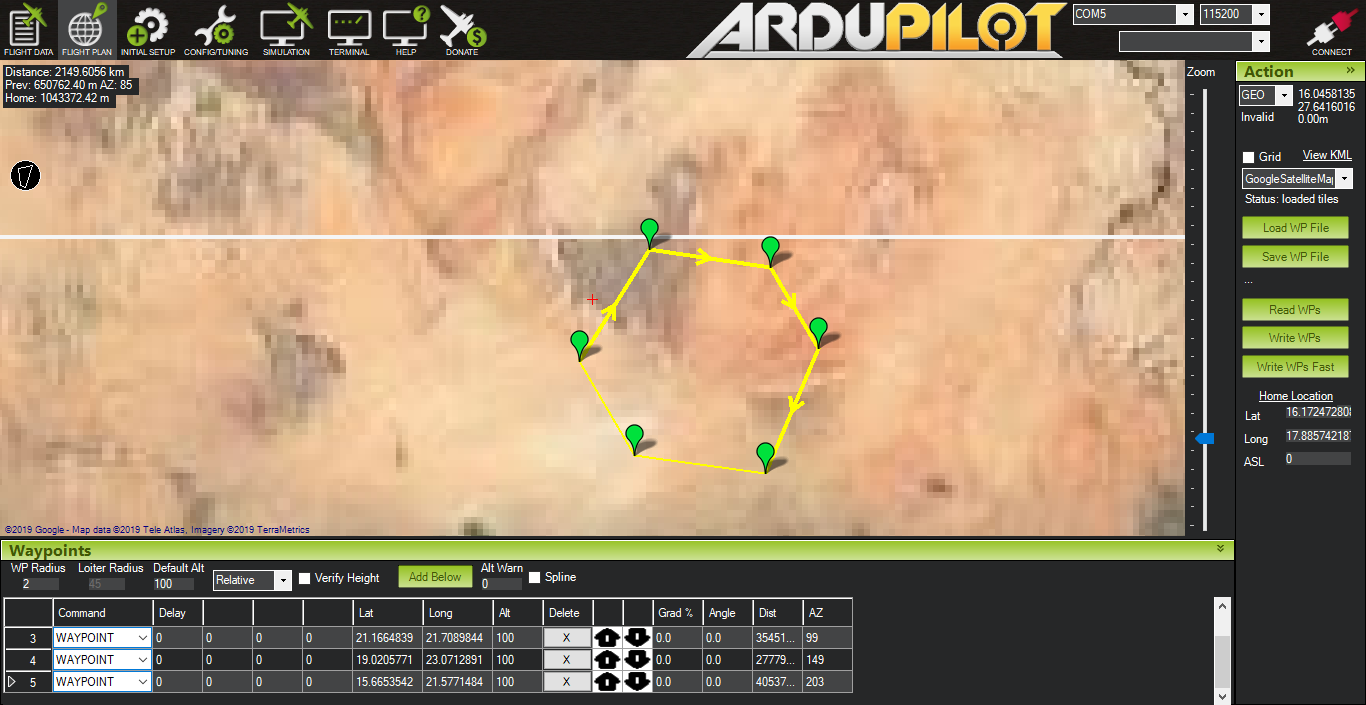
\includegraphics[width=\linewidth]{SummerInterReport/project/Images-Major/mnew.png}
    \caption{Planned Mission}
    \label{fig:compEy}
\end{figure}

\section{Data Acquisition and Processing System}
The Data Acquisition and Processing System consists of a Raspberry Pi 3B model, a Picam version 2 RGB camera and a Pi NoIR Camera. These cameras were used due to their low costs (7\$ and 10\$ respectively), low weight and direct connectivity to Pi's GPU using the CSI port for communication, which makes them the fastest and the best alternatives available. These cameras were located at the bottom of the drone setup in an encasing we designed to keep the set-up expandable and safe on landing.
\\
We tested the two camera system where both of these cameras were used simultaneously to derive the NDVI. In our final work, we have used only the NoIR camera (as shown in the figure below)
\begin{figure}[H]
    \centering
    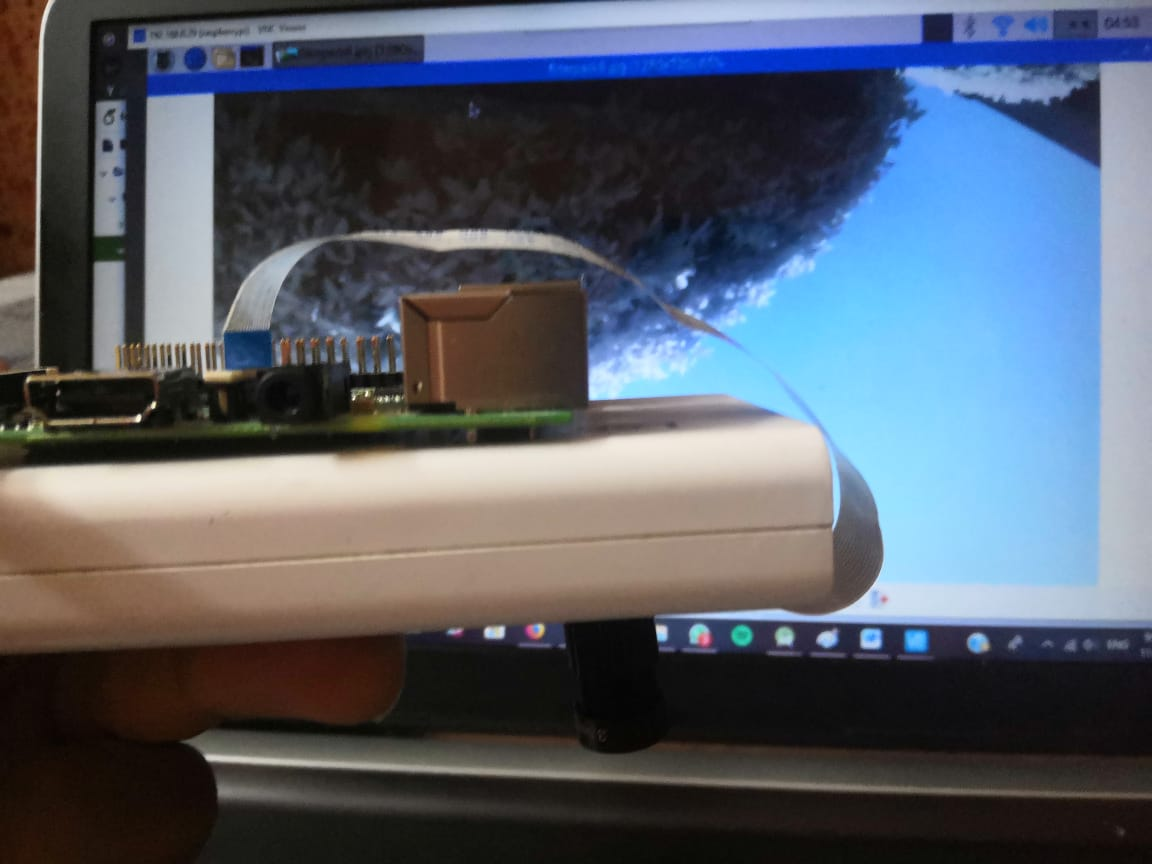
\includegraphics[width=0.7\linewidth]{SummerInterReport/project/Images-Major/pi_system.jpeg}
    \caption{Data Acquisition and Processing System}
    \label{fig:compEy}
\end{figure}

\subsection{Raspberry Pi}
 The Raspberry Pi is used to collect the data and act as the trigger. It detects the trigger event by the flight controller and then capture images with time and GPS stamp. Raspberry Pi 3B is a microcomputer which can run on any compact OS. We selected the native Raspbian OS to operate the Pi. We used the high speed CSI port (Camera Serial Interface). It is a specification of the Mobile Industry Processor Interface (MIPI) Alliance. It defines an interface between a camera and a host processor. The CSI port in Pi connects the camera directly with the VideoCore IV GPU of the Raspberry Pi.
 \begin{figure}[H]
    \centering
    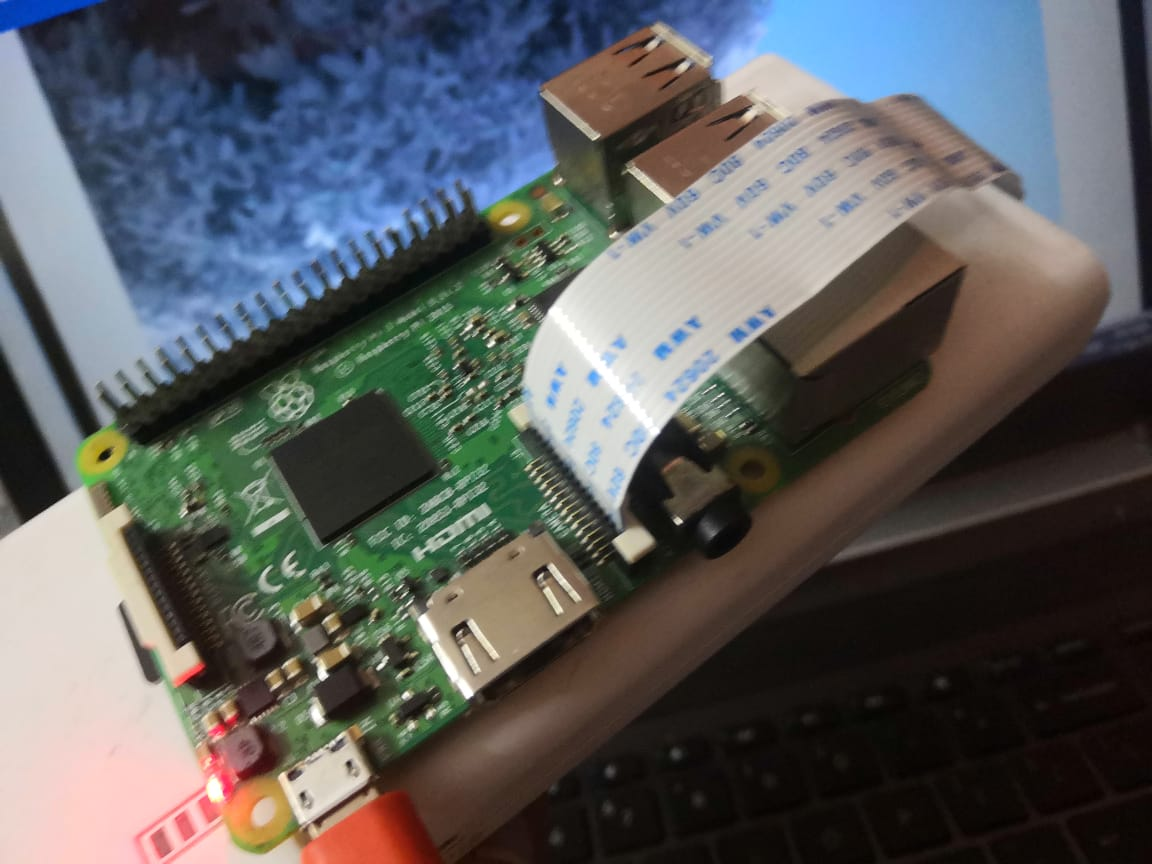
\includegraphics[width=0.5\linewidth]{SummerInterReport/project/Images-Major/pi_top.jpeg}
    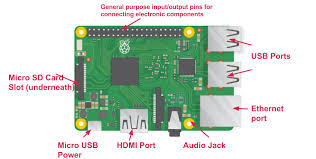
\includegraphics[width=0.5\linewidth]{SummerInterReport/project/Images-Major/pi.jpg}
    \caption{RaspberryPi 3B}
    \label{fig:compEy}
\end{figure}
 The 3B model of Raspberry Pi has the following specifications relevant for data processing and acquisition:
 \begin{itemize}
     \item Quad Core 1.2GHz Broadcom BCM2837 64bit CPU
     \item 1GB RAM
     \item BCM43438 wireless LAN and Bluetooth Low Energy (BLE) on board for communication purposes for live feed analysis.
     \item 40-pin extended GPIO
     \item CSI camera port for connecting a Raspberry Pi camera
     \item Micro SD port for loading your operating system and storing data
     \item 4 USB 2 ports
 \end{itemize}
\subsection{NoIR Camera}
The Pi NoIR gives everything the regular RGB Camera Module offers, with one difference: it does not employ an infrared filter. (NoIR = No Infrared.) This means that pictures we take contains the Near Infra Red component in the taken pictures. We also employ a red light filter to block off all extra incoming light. The sensor used is a 5-megapixel OmniVision OV5647 sensor.
\begin{figure}[H]
    \centering
    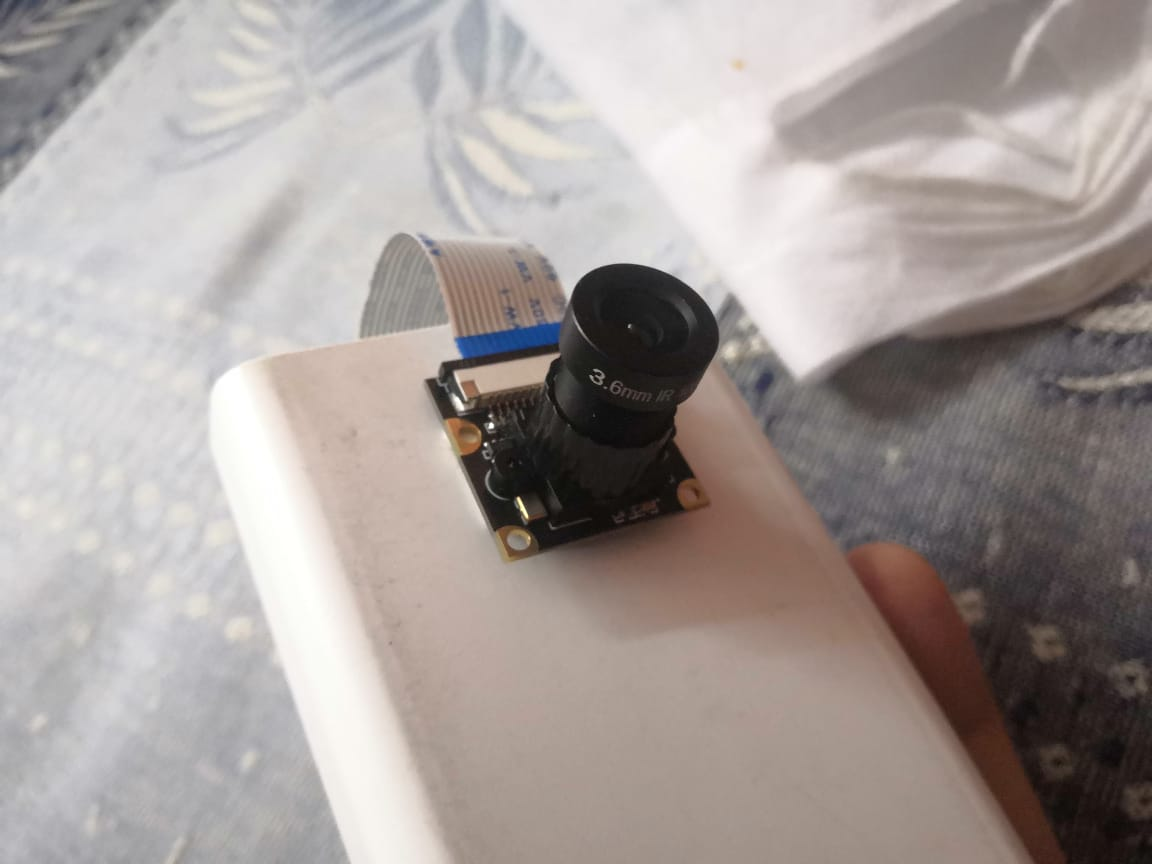
\includegraphics[width=0.7\linewidth]{SummerInterReport/project/Images-Major/pi_bottom.jpeg}
    \caption{NoIR Camera}
    \label{fig:compEy}
\end{figure}
\section{Android Application}
Android Application is responsible for connecting the farmer to drone service facility. We deployed a simple user interface to communicate with the user and connect them with the drone. The application provides field related infographics like live streaming of NDVI calculation while the drone is analyzing the field, presenting past post-processed infographics and calling for the drone service
The android application contains the following components:
\subsection{Calling the Drone Service}- The drone service call is made using the Firebase realtime database. Firebase is a cloud solution by Google which provides functionality like realtime messages with latency as low as 25ms, Storages and online ML kits. The application firstly fetches the GPS coordinates of the phone, and hence the user (Latitude, Longitude and Altitude). These are updated over the realtime cloud database as a unique entry in the Tree Database, using the phone's MAC address to identify it. This reduces the manual complex sign-in process in order to avoid confusion with the farmer. This location is programmed to the drone at the drone dispatching station or the base station, along with making the coverage polygon.
\subsection{Past post processed reports} The application provisions the storage of past reports and the post flight processing reports on the Storage Database by Firebase which is used as a back-end server. The stored information is related to the previous health monitoring report of crop field, which can help in the validation of the crop health by comparing the current and the previous report of the crop field.

\subsection{Live Analysis}We use web streaming over a given WLAN IP and port, wherein, mobile jpg (.mjpg) format images are updated at fast refresh rates to communicate over the whole captured and computed video, thereby working as live-streaming. Thisis displayed in the application using a WebView.


\subsection{Hindi Translation}The application uses Hindi Text views and Buttons to support Bilungistic approach. For language translation, we use Unicode characters supported by Android devices and toggling of language is done through a public binary flag variable which is accessed throughout the application from the MainActivity.java

\begin{figure}[H]
    \centering
    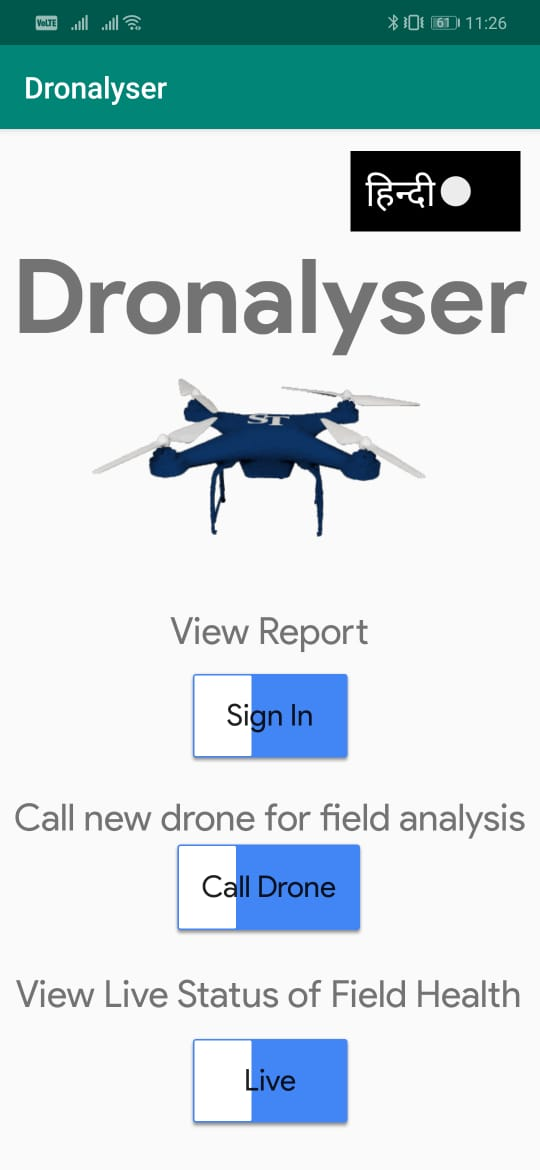
\includegraphics[scale=0.17]{SummerInterReport/project/Images-Major/app1.jpeg}
    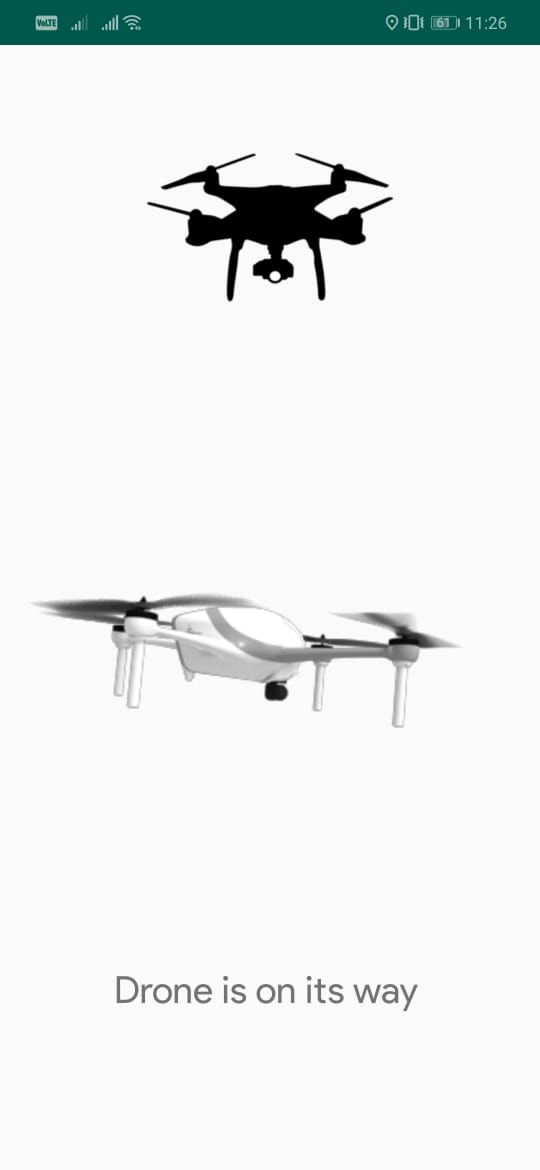
\includegraphics[scale=0.17]{SummerInterReport/project/Images-Major/app2.jpeg}
    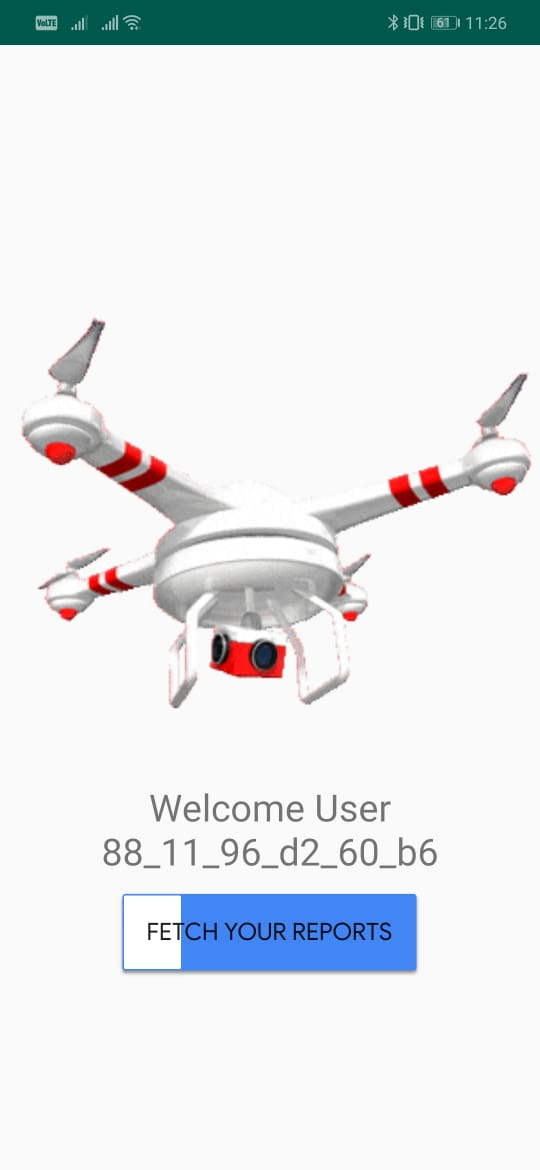
\includegraphics[scale=0.17]{SummerInterReport/project/Images-Major/app3.jpeg}
    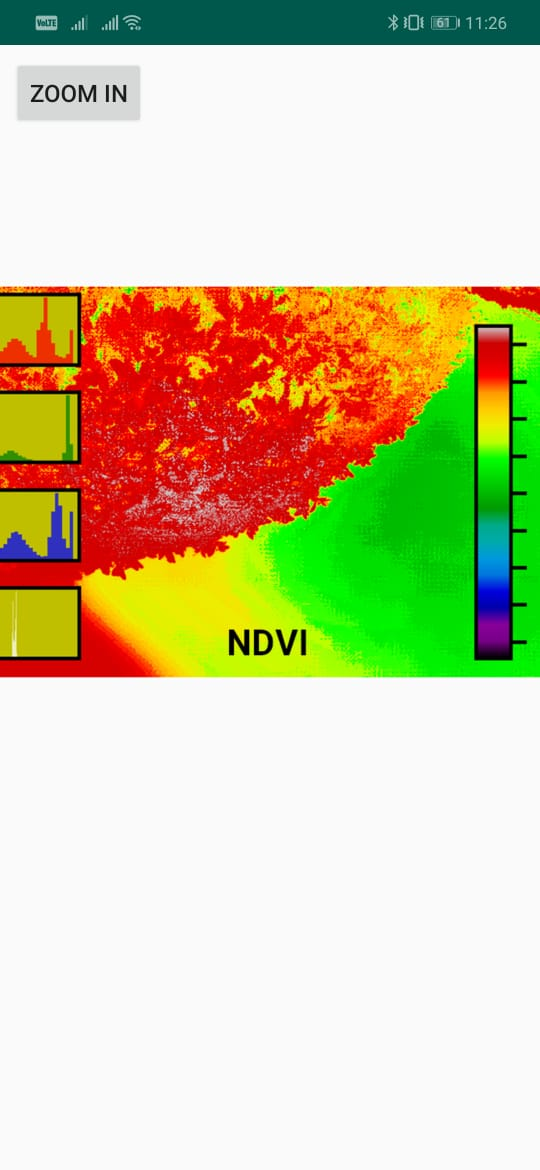
\includegraphics[scale=0.17]{SummerInterReport/project/Images-Major/app4.jpeg}
    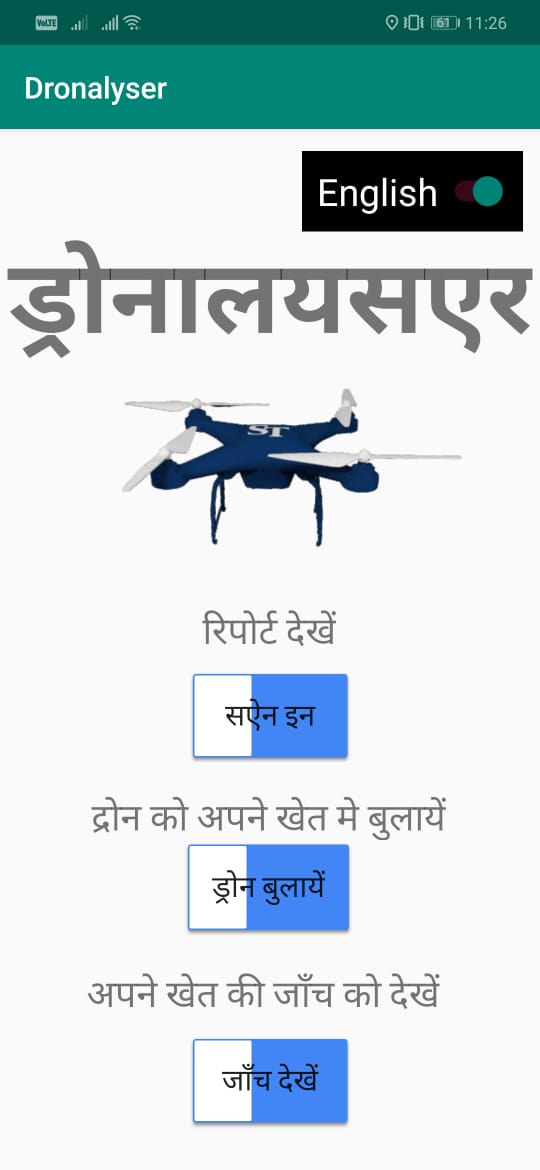
\includegraphics[scale=0.17]{SummerInterReport/project/Images-Major/app5.jpeg}
    \caption{Application Screenshots}
    \label{fig:compEy}
\end{figure}

\subsection{Snippets}
\newpage
\textbf{Fetching location}
\begin{lstlisting}[language=Java]
public void getLoc() {
        lm = (LocationManager)
                getSystemService(Context.LOCATION_SERVICE);
        locationListener = new MyLocationListener();
        Location loc = null;
        TextView droneText = (TextView)findViewById(R.id.droneText);
        try {
            lm.requestLocationUpdates(
                    LocationManager.GPS_PROVIDER,
                    0,
                    0,
                    locationListener);
            loc = lm.getLastKnownLocation(LocationManager.GPS_PROVIDER);
        } catch (SecurityException e) {
            Toast.makeText(getBaseContext(),
                    "Can't access GPS values",
                    Toast.LENGTH_SHORT).show();
        }


        if (loc != null) {
            Loc.setLat(loc.getLatitude());
            Loc.setAlt(loc.getAltitude());
            Loc.setLong(loc.getLongitude());
            FirebaseDatabase database = FirebaseDatabase.getInstance();
            DatabaseReference myRef = database.getReference(macAddr);
            myRef.setValue(Loc);
            droneText.setText("Drone is on its way");
        } 
        else {
            Toast.makeText(getBaseContext(),
                    "Location is null",
                    Toast.LENGTH_SHORT).show();
        }
}
\end{lstlisting}
\textbf{Fetching reports}
\begin{lstlisting}[language=Java]
storageReference.child(nameMacAddr + ".png").getBytes(Long.MAX_VALUE).addOnSuccessListener(new OnSuccessListener<byte[]>() {
            @Override
            public void onSuccess(byte[] bytes) {
                // Use the bytes to display the image
                bmptoimg.setImageViewWithByteArray(reportImage,bytes);
            }
        }).addOnFailureListener(new OnFailureListener() {
            @Override
            public void onFailure(@NonNull Exception exception) {
                // Handle any errors
            }
});
\end{lstlisting}
